%-*-latex-*-
\section{Linked List Diagrams}

\usetikzlibrary{calc,shapes.multipart,chains,arrows}
%\usetikzlibrary{matrix}
%\usetikzlibrary{decorations.pathmorphing}
%\usetikzlibrary{decorations.text}
%\usetikzlibrary{decorations.shapes}
%\usetikzlibrary{decorations.fractals}
%\usetikzlibrary{decorations.footprints}
%\usetikzlibrary{shapes.gates.logic.US,trees,positioning,arrows}



\[
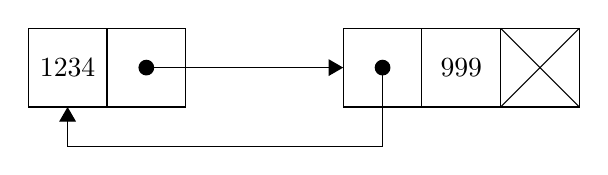
\begin{tikzpicture}[>=triangle 60]

\draw (1,0) rectangle (2,1);   % mid square
\draw (1.5,0.5) node {$1234$}; % data
\draw (2,0) rectangle (3,1);   % right square

\fill     (2.5, 0.5) circle (0.1cm); % right arrow
\draw[->] (2.5, 0.5) -- (5.0, 0.5);

\draw (5,0) rectangle (6,1);
\draw (6,0) rectangle (7,1);
\draw (6.5,0.5) node {$999$}; % data
\draw (7,0) rectangle (8,1);

\draw[->] (5.5, 0.5) -- (5.5, -0.5) -- (1.5, -0.5) -- (1.5, 0.0);
\fill     (5.5, 0.5) circle (0.1cm);

\draw (7,0) -- (8,1);
\draw (7,1) -- (8,0);

\end{tikzpicture}
\]


\[
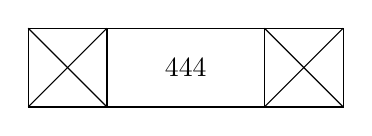
\begin{tikzpicture}[>=triangle 60]

\draw (0, 0) rectangle (1, 1);
\draw (1, 0) rectangle (3, 1);
\draw (2.0, 0.5) node {444};
\draw (3, 0) rectangle (4, 1);

\draw (0, 1) -- (1, 0);
\draw (0, 0) -- (1, 1);
        
\draw (3, 0) -- (4, 1);
\draw (3, 1) -- (4, 0);
        
\end{tikzpicture}
\]


\newpage

{\bf TEST DEFAULT NEXT PATH:}
\\

Next is EAST: \\

\begin{tikzpicture}[>=triangle 60]
\bShell[python 1>abc.txt 2>abc.txt]
from latex_ds import * 

a = dllist([0,1], points=[[0,0],[3,0]])
a[0].setnext(a[1])
a[1].setprev(None)
for i in range(len(a)): print(a[i])

\eShell\input{abc.txt}
\end{tikzpicture}
\mbox{}\\ \\

Next is NORTHEAST: \\

\begin{tikzpicture}[>=triangle 60]
\bShell[python 1>abc.txt 2>abc.txt]
from latex_ds import * 

a = dllist([0,1], points=[[0,0],[3,1]])
a[0].setnext(a[1])
a[1].setprev(None)
for i in range(len(a)): print(a[i])

\eShell\input{abc.txt}
\end{tikzpicture}
\mbox{}\\ \\

Next is SOUTHEAST: \\

\begin{tikzpicture}[>=triangle 60]
\bShell[python 1>abc.txt 2>abc.txt]
from latex_ds import * 

a = dllist([0,1], points=[[0,0],[3,-1]])
a[0].setnext(a[1])
a[1].setprev(None)
for i in range(len(a)): print(a[i])

\eShell\input{abc.txt}
\end{tikzpicture}
\mbox{}\\ \\

Next is NORTHWEST: 
\\

\begin{tikzpicture}[>=triangle 60]
\bShell[python 1>abc.txt 2>abc.txt]
from latex_ds import * 

a = dllist([0,1], points=[[0,0],[-3,1]])
a[0].setnext(a[1])
a[1].setprev(None)
for i in range(len(a)): print(a[i])

\eShell\input{abc.txt}
\end{tikzpicture}
\mbox{}\\ \\

Next is WEST:
\\

\begin{tikzpicture}[>=triangle 60]
\bShell[python 1>abc.txt 2>abc.txt]
from latex_ds import * 

a = dllist([0,1], points=[[0,0],[-3,0]])
a[0].setnext(a[1])
a[1].setprev(None)
for i in range(len(a)): print(a[i])

\eShell\input{abc.txt}
\end{tikzpicture}
\mbox{}\\ \\

Next is SOUTHWEST:
\\

\begin{tikzpicture}[>=triangle 60]
\bShell[python 1>abc.txt 2>abc.txt]
from latex_ds import * 

a = dllist([0,1], points=[[0,0],[-3,-1]])
a[0].setnext(a[1])
a[1].setprev(None)
for i in range(len(a)): print(a[i])

\eShell\input{abc.txt}
\end{tikzpicture}
\mbox{}\\ \\


Next is NORTH: \\

\begin{tikzpicture}[>=triangle 60]
\bShell[python 1>abc.txt 2>abc.txt]
from latex_ds import * 

a = dllist([0,1], points=[[0,0],[0,2]])
a[0].setnext(a[1])
a[1].setprev(None)
for i in range(len(a)): print(a[i])

\eShell\input{abc.txt}
\end{tikzpicture}
\mbox{}\\ \\


Next is SOUTH: \\

\begin{tikzpicture}[>=triangle 60]
\bShell[python 1>abc.txt 2>abc.txt]
from latex_ds import * 

a = dllist([0,1], points=[[0,0],[0,-2]])
a[0].setnext(a[1])
a[1].setprev(None)
for i in range(len(a)): print(a[i])

\eShell\input{abc.txt}
\end{tikzpicture}
\mbox{}\\ \\

Next is self: \\

\begin{tikzpicture}[>=triangle 60]
\bShell[python 1>abc.txt 2>abc.txt]
from latex_ds import * 

a = dllist([0], points=[[0,0]])
a[0].setnext(a[0])
for i in range(len(a)): print(a[i])

\eShell\input{abc.txt}
\end{tikzpicture}
\mbox{}\\ \\

\newpage


{\bf TEST DEFAULT PREV PATH:}
\\

Prev is WEST [OK]: \\

\begin{tikzpicture}[>=triangle 60]
\bShell[python 1>abc.txt 2>abc.txt]
from latex_ds import * 

a = dllist([0,1], points=[[0,0],[3,0]])
a[0].setnext(None)
a[1].setprev(a[0])
for i in range(len(a)): print(a[i])

\eShell\input{abc.txt}
\end{tikzpicture}
\mbox{}\\ \\

Prev is SOUTHWEST [OK]: \\

\begin{tikzpicture}[>=triangle 60]
\bShell[python 1>abc.txt 2>abc.txt]
from latex_ds import * 

a = dllist([0,1], points=[[0,0],[3,1]])
a[0].setnext(None)
a[1].setprev(a[0])
for i in range(len(a)): print(a[i])

\eShell\input{abc.txt}
\end{tikzpicture}
\mbox{}\\ \\

Prev is NORTHWEST [OK]: \\

\begin{tikzpicture}[>=triangle 60]
\bShell[python 1>abc.txt 2>abc.txt]
from latex_ds import * 

a = dllist([0,1], points=[[0,0],[3,-1]])
a[0].setnext(None)
a[1].setprev(a[0])
for i in range(len(a)): print(a[i])

\eShell\input{abc.txt}
\end{tikzpicture}
\mbox{}\\ \\

Prev is SOUTHEAST: 
\\

\begin{tikzpicture}[>=triangle 60]
\bShell[python 1>abc.txt 2>abc.txt]
from latex_ds import * 

a = dllist([0,1], points=[[0,0],[-3,1]])
a[0].setnext(None)
a[1].setprev(a[0])
for i in range(len(a)): print(a[i])

\eShell\input{abc.txt}
\end{tikzpicture}
\mbox{}\\ \\

Prev is EAST:
\\

\begin{tikzpicture}[>=triangle 60]
\bShell[python 1>abc.txt 2>abc.txt]
from latex_ds import * 

a = dllist([0,1], points=[[0,0],[-3,0]])
a[0].setnext(None)
a[1].setprev(a[0])
for i in range(len(a)): print(a[i])

\eShell\input{abc.txt}
\end{tikzpicture}
\mbox{}\\ \\

Prev is NORTHEAST:
\\

\begin{tikzpicture}[>=triangle 60]
\bShell[python 1>abc.txt 2>abc.txt]
from latex_ds import * 

a = dllist([0,1], points=[[0,0],[-3,-1]])
a[0].setnext(None)
a[1].setprev(a[0])
for i in range(len(a)): print(a[i])

\eShell\input{abc.txt}
\end{tikzpicture}
\mbox{}\\ \\


Prev is SOUTH: \\

\begin{tikzpicture}[>=triangle 60]
\bShell[python 1>abc.txt 2>abc.txt]
from latex_ds import * 

a = dllist([0,1], points=[[0,0],[0,2]])
a[0].setnext(None)
a[1].setprev(a[0])
for i in range(len(a)): print(a[i])

\eShell\input{abc.txt}
\end{tikzpicture}
\mbox{}\\ \\


Prev is NORTH: \\

\begin{tikzpicture}[>=triangle 60]
\bShell[python 1>abc.txt 2>abc.txt]
from latex_ds import * 

a = dllist([0,1], points=[[0,0],[0,-2]])
a[0].setnext(None)
a[1].setprev(a[0])
for i in range(len(a)): print(a[i])

\eShell\input{abc.txt}
\end{tikzpicture}
\mbox{}\\ \\

Prev is self: \\

\begin{tikzpicture}[>=triangle 60]
\bShell[python 1>abc.txt 2>abc.txt]
from latex_ds import * 

a = dllist([0], points=[[0,0]])
a[0].setprev(a[0])
for i in range(len(a)): print(a[i])

\eShell\input{abc.txt}
\end{tikzpicture}
\mbox{}\\ \\

\newpage




\begin{flushleft}
{\bf INSERTION.}
\end{flushleft}

Here is a doubly linked list in the heap.
\[
\begin{tikzpicture}[>=triangle 60]
\bShell[python 1>abc.txt 2>abc.txt]
from latex_ds import * 
print(rect(-0.5, -1, 11.5, 1))

n = dllist([0,1,3,4])
for i in range(len(n)): print(n[i])

\eShell\input{abc.txt}
\end{tikzpicture}
\]
We want to add 2 to this double linked list.
In other words we want the following:
\[
\begin{tikzpicture}[>=triangle 60]
\bShell[python 1>abc.txt 2>abc.txt]
from latex_ds import * 

print(rect(-0.5, -1, 14.5, 1))

n = dllist([0,1,2,3,4])
for x in n: print(x)

\eShell\input{abc.txt}
\end{tikzpicture}
\]
Suppose that we have the pointer to the node after which
we need to attach a node with key = 2,
say, the pointer to the node (with key = 1) is \verb!p!.
\\ \\



\begin{flushleft}
STEP 1:
First we allocate memory for the new node, say the pointer 
to this new node is \verb!q!.
\end{flushleft}
\[
\begin{tikzpicture}[>=triangle 60]
\bShell[python 1>abc.txt 2>abc.txt]
from latex_ds import * 

print(rect(-1, -2.5, 13, 1))

n = dllist([0,1,3,4], points=[[0,0],[3,0],[7,0],[10,0]])
n0 = DLLISTNODE(x=5, y=-2.0, width=1, height=0.5, key=2, color='red')

for i in range(len(n)): print(n[i])
print(n0)

\eShell\input{abc.txt}
\end{tikzpicture}
\]
The code is
\begin{Verbatim}[frame=single,fontsize=\footnotesize]
DoublyLinkedNode q = new DoublyLinkedNode(2);
\end{Verbatim}
\mbox{}\\ \\







\begin{flushleft}
STEP 2:
\end{flushleft}
\[
\begin{tikzpicture}[>=triangle 60]
\bShell[python 1>abc.txt 2>abc.txt]
from latex_ds import * 

print(rect(-1, -3, 13, 1))

n = dllist([0,1,3,4], points=[[0,0],[3,0],[7,0],[10,0]])
n0 = DLLISTNODE(x=5, y=-2.0, width=1, height=0.5, key=2, color='red')

n[2].setprev(n0, color='red')

for i in range(len(n)): print(n[i])
print(n0)

\eShell\input{abc.txt}
\end{tikzpicture}
\]
The code is:
\begin{Verbatim}[frame=single,fontsize=\footnotesize]
p->next->prev = q;
\end{Verbatim}
\mbox{}\\ \\







\begin{flushleft}
STEP 3:
\end{flushleft}
\[
\begin{tikzpicture}[>=triangle 60]
\bShell[python 1>abc.txt 2>abc.txt]
from latex_ds import * 

print(rect(-1, -3, 13, 1))

n = dllist([0,1,3,4], points=[[0,0],[3,0],[7,0],[10,0]])
n0 = DLLISTNODE(x=5, y=-2.0, width=1, height=0.5, key=2, color='red')

n[2].setprev(n0, color='red')
n0.setnext(n[2], color='red')

for i in range(len(n)): print(n[i])
print(n0)

\eShell\input{abc.txt}
\end{tikzpicture}
\]
The code is
\begin{Verbatim}[frame=single,fontsize=\footnotesize]
q->next = p->next;
\end{Verbatim}
\mbox{}\\ \\





\begin{flushleft}
STEP 4:
\end{flushleft}
\[
\begin{tikzpicture}[>=triangle 60]
\bShell[python 1>abc.txt 2>abc.txt]
from latex_ds import * 

print(rect(-1, -3, 13, 1))

n = dllist([0,1,3,4], points=[[0,0],[3,0],[7,0],[10,0]])
n0 = DLLISTNODE(x=5, y=-2.0, width=1, height=0.5, key=2, color='red')

n[2].setprev(n0, color='red') 
n0.setnext(n[2], color='red')
n[1].setnext(n0, color='red')

for i in range(len(n)): print(n[i])
print(n0)

\eShell\input{abc.txt}
\end{tikzpicture}
\]
The code is
\begin{Verbatim}[frame=single,fontsize=\footnotesize]
p->next = q;
\end{Verbatim}
\mbox{}\\ \\




\begin{flushleft}
STEP 5:
\end{flushleft}
\[
\begin{tikzpicture}[>=triangle 60]
\bShell[python 1>abc.txt 2>abc.txt]
from latex_ds import * 

print(rect(-1, -3, 13, 1))

n = dllist([0,1,3,4], points=[[0,0],[3,0],[7,0],[10,0]])
n0 = DLLISTNODE(x=5, y=-2.0, width=1, height=0.5, key=2, color='red')

n[2].setprev(n0, color='red') 
n0.setnext(n[2], color='red')
n[1].setnext(n0, color='red')
n0.setprev(n[1], 'red')

for i in range(len(n)): print(n[i])
print(n0)

\eShell\input{abc.txt}
\end{tikzpicture}
\]
The code is
\begin{Verbatim}[frame=single,fontsize=\footnotesize]
q->prev = p;
\end{Verbatim}
\mbox{}\\ \\






The result is that we now have the following double linked
list:
\[
\begin{tikzpicture}[>=triangle 60]
\bShell[python 1>abc.txt 2>abc.txt]
from latex_ds import * 

print(rect(-0.5, -1, 14.5, 1))

n = dllist([0,1,2,3,4])
for x in n: print(x)

\eShell\input{abc.txt}
\end{tikzpicture}
\]





\newpage

\begin{flushleft}
{\bf DELETION.}
\end{flushleft}


Here is a doubly linked list in the heap.
\[
\begin{tikzpicture}[>=triangle 60]
\bShell[python 1>abc.txt 2>abc.txt]
from latex_ds import * 

print(rect(-0.5, -1, 14.5, 1))
n = dllist([0,1,2,3,4])
for i in range(len(n)): print(n[i])

\eShell\input{abc.txt}
\end{tikzpicture}
\]
We want to remove the node with key = 2.
In other words, we want this:
\[
\begin{tikzpicture}[>=triangle 60]
\bShell[python 1>abc.txt 2>abc.txt]
from latex_ds import * 
print(rect(-0.5, -1, 11.5, 1))

n = dllist([0,1,3,4])
for i in range(len(n)): print(n[i])

\eShell\input{abc.txt}
\end{tikzpicture}
\]
Suppose the \verb!p! is a pointer that points to the node to be removed.
\\ \\


\begin{flushleft}
STEP 1: Set the next pointer of the node before the node to be deleted.
\end{flushleft}
\[
\begin{tikzpicture}[>=triangle 60]
\bShell[python 1>abc.txt 2>abc.txt]
from latex_ds import * 
import pickle

n = dllist([0,1,2,3,4])
n[1].setnext(n[3], color='red', description='up 0.75')

print(rect(-0.5, -1, 14.5, 1.5))
for i in range(5): print(n[i])

pickle.dump(n, open('n.pkl', 'w'))
\eShell\input{abc.txt}
\end{tikzpicture}
\]
This means that we need to do this:
\begin{Verbatim}[frame=single,fontsize=\footnotesize]
p->prev->next = p->next;
\end{Verbatim}
\mbox{}\\ \\


\begin{flushleft}
STEP 2: Set the previous pointer of the node after the node to be deleted.
\end{flushleft}
\[
\begin{tikzpicture}[>=triangle 60]
\bShell[python 1>abc.txt 2>abc.txt]
from latex_ds import * 
import pickle

n = pickle.load(open('n.pkl'))
n[3].setprev(n[1], color='red', description='down 1')

# shift the prev pointer of n[3] slightly to avoid overlap
n[3].prev_path.points[2][0] -= 0.2
n[3].prev_path.points[3][0] -= 0.2

print(rect(-0.5, -1.25, 14.5, 1.5))
for i in range(5): print(n[i])

pickle.dump(n, open('n.pkl', 'w'))
\eShell\input{abc.txt}
\end{tikzpicture}
\]
The code is:
\begin{Verbatim}[frame=single,fontsize=\footnotesize]
p->next->prev = p->prev;
\end{Verbatim}
\mbox{} \\ \\ 


\begin{flushleft}
STEP 3: We release the memory for the node with key = 2.
\end{flushleft}
\[
\begin{tikzpicture}[>=triangle 60]
\bShell[python 1>abc.txt 2>abc.txt]
from latex_ds import * 
import pickle

n = pickle.load(open('n.pkl'))
n[1].setnext(n[3], color='red', description='up 0.75')

print(rect(-0.5, -1.25, 14.5, 1.5))
for i in range(5): print(n[i])

\eShell\input{abc.txt}
\end{tikzpicture}
\]
The code is:
\begin{Verbatim}[frame=single,fontsize=\footnotesize]
delete p;
\end{Verbatim}
\mbox{} \\ \\ 





The result is that we get this, i.e. the doubly linked list with 
the node with key 2 removed.
\[
\begin{tikzpicture}[>=triangle 60]
\bShell[python 1>abc.txt 2>abc.txt]
from latex_ds import * 
print(rect(-0.5, -1, 11.5, 1))

n = dllist([0,1,3,4])
for i in range(len(n)): print(n[i])

\eShell\input{abc.txt}
\end{tikzpicture}
\]



\newpage

\[
\begin{tikzpicture}[>=triangle 60]
\bShell[python 1>abc.txt 2>abc.txt]
from latex_ds import * 
print(dllistnode(x=0, y=0, 
                 height=1, width=1,
                 label="$a$",
                 left_null=False, right_null=False,))
print(dllistnode(x=0, y=2, 
                 height=1, width=1,
                 label="$b$",
               left_null=False,
               right_null=False,
               ))
print(pointer([(2.5,2.5), (2.5, 1.5), (1.5, 1.5), (1.5,1)]))
\eShell\input{abc.txt}
\end{tikzpicture}
\]



\newpage

\[
\begin{tikzpicture}[>=triangle 60]
\bShell[python 1>abc.txt 2>abc.txt]
from latex_ds import * 
print(dllistnode(x=0, y=0, 
                 height=1, width=1,
                 label="$a$",
                 left_null=False, right_null=False,))
print(cross(0, -1, 3, 2))
\eShell\input{abc.txt}
\end{tikzpicture}
\]

\newpage

\[
\begin{tikzpicture}[>=triangle 60]
\bShell[python 1>abc.txt 2>abc.txt]

from latex_ds import * 
print(Path(x=0, y= 0, points=[(0,0), (1,1), (2,0)], end="->"))
print(Path(x=0, y=-1, points=[(0,0), (1,1), (2,0)], end="->>"))
print(Path(x=0, y=-2, points=[(0,0), (1,1), (2,0)], end="-|"))
print(Path(x=0, y=-3, points=[(0,0), (1,1), (2,0)], end="-)"))
print(Path(x=0, y=-4, points=[(0,0), (1,1), (2,0)], end="->", color='red'))

print(Rect(x=0,  y=-6, width=1, height=1, color='blue'))
print(CrossedRect(x=0,  y=-7, width=2, height=0.5, color='blue'))
print(Rect(x=0,  y=-9, width=1, height=1, color='blue', text='abc'))

n0 = DLLISTNODE(key=42, x=0, y=-11, width=1, height=0.5)
n1 = DLLISTNODE(key=43, x=4, y=-11, width=1, height=0.5)

n0.setnext(n1)
n1.setprev(n0, color='red')
print(n0)
print(n1)

\eShell\input{abc.txt}
\end{tikzpicture}
\]



\newpage

\begin{tikzpicture}[
% Gates and symbols style
    and/.style={and gate US,thick,draw,fill=red!60,rotate=90,
		anchor=east,xshift=-1mm},
    or/.style={or gate US,thick,draw,fill=blue!60,rotate=90,
		anchor=east,xshift=-1mm},
    be/.style={circle,thick,draw,fill=green!60,anchor=north,
		minimum width=0.7cm},
    tr/.style={buffer gate US,thick,draw,fill=purple!60,rotate=90,
		anchor=east,minimum width=0.8cm},
% Label style
    label distance=3mm,
    every label/.style={blue},
% Event style
    event/.style={rectangle,thick,draw,fill=yellow!20,text width=2cm,
		text centered,font=\sffamily,anchor=north},
% Children and edges style
    edge from parent/.style={very thick,draw=black!70},
    edge from parent path={(\tikzparentnode.south) -- ++(0,-1.05cm)
			-| (\tikzchildnode.north)},
    level 1/.style={sibling distance=7cm,level distance=1.4cm,
			growth parent anchor=south,nodes=event},
    level 2/.style={sibling distance=7cm},
    level 3/.style={sibling distance=6cm},
    level 4/.style={sibling distance=3cm}
%%  For compatability with PGF CVS add the absolute option:
%   absolute
    ]
%% Draw events and edges
    \node (g1) [event] {No flow to receiver}
	     child{node (g2) {No flow from Component B}   
	     	child {node (g3) {No flow into Component B}
	     	   child {node (g4) {No flow from Component A1}
	     	      child {node (t1) {No flow from source1}}
	     	      child {node (b2) {Component A1 blocks flow}}
			}
	     	   child {node (g5) {No flow from Component A2}
	     	      child {node (t2) {No flow from source2}}
	     	      child {node (b3) {Component A2 blocks flow}}
			}
		   }
	     	child {node (b1) {Component B blocks flow}}
		};
%% Place gates and other symbols
%% In the CVS version of PGF labels are placed differently than in PGF 2.0
%% To render them correctly replace '-20' with 'right' and add the 'absolute'
%% option to the tikzpicture environment. The absolute option makes the 
%% node labels ignore the rotation of the parent node. 
   \node [or]	at (g2.south)	[label=-20:G02]	{};
   \node [and]	at (g3.south)	[label=-20:G03]	{};
   \node [or]	at (g4.south)	[label=-20:G04]	{};
   \node [or]	at (g5.south)	[label=-20:G05]	{};
   \node [be]	at (b1.south)	[label=below:B01]	{};
   \node [be]	at (b2.south)	[label=below:B02]	{};
   \node [be]	at (b3.south)	[label=below:B03]	{};
   \node [tr]	at (t1.south)	[label=below:T01]	{};
   \node [tr]	at (t2.south)	[label=below:T02]	{};
%% Draw system flow diagram
   \begin{scope}[xshift=-7.5cm,yshift=-5cm,very thick,
		node distance=1.6cm,on grid,>=stealth',
		block/.style={rectangle,draw,fill=cyan!20},
		comp/.style={circle,draw,fill=orange!40}]
   \node [block] (re)					{Receiver};
   \node [comp]	 (cb)	[above=of re]			{B}  edge [->] (re);
   \node [comp]	 (ca1)	[above=of cb,xshift=-0.8cm]	{A1} edge [->] (cb);
   \node [comp]	 (ca2)	[right=of ca1]			{A2} edge [->] (cb);
   \node [block] (s1)	[above=of ca1]		{Source1} edge [->] (ca1);
   \node [block] (s2)	[right=of s1]		{Source2} edge [->] (ca2);
   \end{scope}
\end{tikzpicture}





\newpage

Alice and Bob is playing a game involving two piles $A$ and $B$ of pebbles.
The game starts with 10 pebbles in each pile.
Alice begins by removing either 
one pebble from exactly one pile or from both.
So Alice has three choices:
\[
(10,10) \rightarrow (9, 10), \hspace{1cm}
(10,10) \rightarrow (10, 9), \hspace{1cm}
(10,10) \rightarrow (9, 9), \hspace{1cm}
\]
Bob then does the same: he can either remove a pebble from eactly one
pile or from both.
The game continues both piles are empty.
The winner is the last to be able to make a move.

Here's the question: If you're Alice, do you have a winning strategy?
Or if you're Bob, do you have a winner strategy?

Let's start simple and work with two piles of 2 pebbles
... and hope that what we can discover somehow translates to the case
of two piles of 10 pebbles each.
Here's the complete decision tree for this game:
\[
\begin{tikzpicture}[>=triangle 60]
{\tiny
\bShell[python 1>abc.txt 2>abc.txt]
from latex_ds import * 
print(tree(skip_key='',
    keys=['2,2',
    '1,2', '2,1', '1,1', 
    '0,2', '1,1', '0,1',
    '1,1', '2,0', '1,0', 
    '0,1', '1,0', '0,0', 
    '',   '0,1', '', 
    '0,1', '1,0', '0,0',
    '',   '0,0', '',
    '0,1', '1,0', '0,0',
    '',   '1,0', '', 
    '0,0', '',   '',
    '',   '0,0', '',
    '0,0', '',   '',
    '',   '',   '',
    '',   '',   '',
    '',   '0,0', '',
    '',   '',   '',
    '',   '0,0', '',
    '0,0',  '',  '',
    '',    '',  '',
    '',    '',  '',
    '',    '',  '',
    '','','',
    '',    '0,0', '',
    '0,0','','',
    '','','',
'','','',
'','0,0','',
]))
\eShell\input{abc.txt}
}
\end{tikzpicture}
\]
If you look at this carefully, you'd see that Alice does not have a 100\%
foolproof winning strategy.
However note that Bob {\it does} have a winning strategy.
\begin{enumerate}
\item If Alice picks one pebble from the first pile, Bob will pick one pebble
      from the first file.
\item If Alice picks one pebble from the second pile, Bob will pick one
      pebble from the second pile.
\item If Alice picks one pebble from each pile, then Bob will pick
      one pebble from each pile.
\end{enumerate}

Let's try to organize the data in a different way.
Here's a grid (instead of a tree) where the row and column gives you
the number of pebbles in the first and second pile:
\begin{longtable}{|c|ccc|} \hline
  & 0 & 1 & 2 \\
\hline
0 &  &  &  \\
1 &  &  &  \\
2 &  &  &  \\
\hline
\end{longtable}
The table tells you what you should do in order to win 
if there's a winning strategy and it tells you when you do not have
a winning strategy.
Let's use $*$ to denote there's no winning strategy.
So in the $(2,2)$ cell we put a $*$:
\begin{longtable}{|c|ccc|} \hline
  & 0 & 1 & 2 \\
\hline
0 &  &  &  \\
1 &  &  &  \\
2 &  &  &  $*$ \\
\hline
\end{longtable}
If you are looking at $(0,0)$, i.e. no more pebbles left,
then of course you have lost; your opponent just made the last
move to empty both piles:
\begin{longtable}{|c|ccc|} \hline
  & 0 & 1 & 2 \\
\hline
0 & $*$ &  &  \\
1 &  &  &  \\
2 &  &  &  $*$ \\
\hline
\end{longtable}
Now let's look at case of $(1,2)$. 
Pretend you're Bob.
What would you do you have 1 pebble in the first pile and
2 in the second?
Look at the decision tree with node labeled $(1,2)$.
You see that you should take one pebble from the first pile
to reach $(0,2)$ in order to guarantee a win:
\begin{longtable}{|c|ccc|} \hline
  & 0   & 1 & 2 \\ \hline
0 & $*$ &   &  \\
1 &     &   &  $\uparrow$ \\
2 &     &   &  $*$ \\
\hline
\end{longtable}
The up arrow $\uparrow$ in $(1,2)$ tells me to go to the cell
at $(0,2$).
By symmetry we have the following at $(2,1)$:
\begin{longtable}{|c|ccc|} \hline
  & 0   & 1 & 2 \\ \hline
0 & $*$ &   &  \\
1 &     &   &  $\uparrow$ \\
2 &     & $\leftarrow$  &  $*$ \\
\hline
\end{longtable}
If you look at the decision tree at $(1,1)$,

Now look at the node with $(1,1)$ in the decision tree.
You win immediately if you remove one pebble from 
each pile to reach $(0,0)$:
\begin{longtable}{|c|ccc|} \hline
  & 0   & 1 & 2 \\ \hline
0 & $*$ &   &  \\
1 &     & $\nwarrow$&  $\uparrow$ \\
2 &     & $\leftarrow$  &  $*$ \\
\hline
\end{longtable}
The northwest arrow $\nwarrow$ at $(1,1)$ tells me to go to
$(0,0)$ (i.e., remove one pebble from each pile).

We have 4 empty cells left. 
Don't forget that by symmetry we only need to know to do with 2 of them.

Let's look at $(0,1)$.
Of course you remove a pebble from the second pile.
(See the decision tree.)
Likewise if you're at $(1,0)$, you remove the pebble in the first pile.
\begin{longtable}{|c|ccc|} \hline
  & 0   & 1 & 2 \\ \hline
0 & $*$ & $\leftarrow$  &  \\
1 & $\uparrow$    & $\nwarrow$&  $\uparrow$ \\
2 &     & $\leftarrow$  &  $*$ \\
\hline
\end{longtable}

Now for $(0,2)$.
The decision tree tells you that you have no winning strategy.
Same thing happens at $(2,0)$.
So here's the completed grid:
\begin{longtable}{|c|ccc|} \hline
  & 0   & 1 & 2 \\ \hline
0 & $*$ & $\leftarrow$  &  $*$ \\
1 & $\uparrow$    & $\nwarrow$&  $\uparrow$ \\
2 & $*$ & $\leftarrow$  &  $*$ \\
\hline
\end{longtable}
There's obviously some kind of pattern here.
Maybe this happens for a 3-by-3 grid too???
\begin{longtable}{|c|cccc|} \hline
  & 0   & 1 & 2 & 3\\ \hline
0 & $*$ & $\leftarrow$  &  $*$ & \\
1 & $\uparrow$    & $\nwarrow$&  $\uparrow$ & \\
2 & $*$ & $\leftarrow$  &  $*$ & \\
3 &     &               &      & \\ \hline
\end{longtable}

Let's look at $(3,0)$.
We can remove a pebble from the first pile to reach $(2,0)$
which will force our opponent {\it not} to have a winning strategy.
The same idea applies to $(0,3)$.
So we get
\begin{longtable}{|c|cccc|} \hline
  & 0   & 1 & 2 & 3\\ \hline
0 & $*$ & $\leftarrow$  &  $*$ & $\leftarrow$ \\
1 & $\uparrow$    & $\nwarrow$&  $\uparrow$ & \\
2 & $*$ & $\leftarrow$  &  $*$ & \\
3 & $\uparrow$    &               &      & \\ \hline
\end{longtable}

At $(3,1)$, using the same idea, we can get to $(2,0)$ by
removing one pebble from each pile and at $(2,0)$ we see that
our opponent does not have a winning strategy (like above).
Same idea applies to $(1,3)$.
\newpage
\begin{longtable}{|c|cccc|} \hline
  & 0   & 1 & 2 & 3\\ \hline
0 & $*$ & $\leftarrow$  &  $*$ & $\leftarrow$ \\
1 & $\uparrow$    & $\nwarrow$&  $\uparrow$ & $\nwarrow$ \\
2 & $*$ & $\leftarrow$  &  $*$ & \\
3 & $\uparrow$    & $\nwarrow$              &      & \\ \hline
\end{longtable}

At $(3,2)$ or $(2,3)$ we move to the closest $*$ at $(2,2)$ 
to force our opponent to {\it not} have a winning strategy:
\begin{longtable}{|c|cccc|} \hline
  & 0   & 1 & 2 & 3\\ \hline
0 & $*$ & $\leftarrow$  &  $*$ & $\leftarrow$ \\
1 & $\uparrow$    & $\nwarrow$&  $\uparrow$ & $\nwarrow$ \\
2 & $*$ & $\leftarrow$  &  $*$ & $\leftarrow$ \\
3 & $\uparrow$    & $\nwarrow$ & $\uparrow$ & \\ \hline
\end{longtable}

At $(3,3)$ we can go to $(2,2)$ (where our opponent does not have
a winning strategy) by removing one pebble from each pile:
\begin{longtable}{|c|cccc|} \hline
  & 0   & 1 & 2 & 3\\ \hline
0 & $*$ & $\leftarrow$  &  $*$ & $\leftarrow$ \\
1 & $\uparrow$    & $\nwarrow$&  $\uparrow$ & $\nwarrow$ \\
2 & $*$ & $\leftarrow$  &  $*$ & $\leftarrow$ \\
3 & $\uparrow$    & $\nwarrow$ & $\uparrow$ & $\nwarrow$ \\ \hline
\end{longtable}

{\bf Exercise.}
Draw the grid for 4-by-4.
Check that it makes sense.
When you're confident ... Draw the grid for 10-by-10.

Once you have a couple of grids, you would realize that the
easier cells to fill are the ones on the boundary, i.e.,
the ones that correspond to cases where one pile is empty, i.e.
the cell at
\[
(0, j)
\]
or 
\[
(i, 0)
\]
If $R_{i,j}$ denotes the value at $(i,j)$ then
\[
R_{i,j} =
\begin{cases}
*          & \text{if $i = 0$ and $j$ is even} \\
\leftarrow & \text{if $i = 0$ and $j$ is odd}  \\ 
*          & \text{if $i$ is even and $j = 0$} \\
\uparrow   & \text{if $i$ is odd and $j = 0$}  \\ 
\end{cases}
\]
What about in general? 
What is the value of $R_{i,j}$ is both $i$ and $j$ are not zero?
If you think 
\[
R_{i,j} = \, \uparrow
\]
then this implies that $R_{i-1,j}$ must have a $*$, this
makes sense only when $i > 0$.
Vice versa if 
\[
R_{i-1, j} = *
\]
then $R_{i,j} = \, \uparrow$.
If you think
\[
R_{i,j} = \, \leftarrow
\]
then this implies that $R_{i, j-1}$ must be a $*$; of course
this makes sense only if $j > 0$.
If you think
\[
R_{i,j} = \, \nwarrow
\]
then this implies that $R_{i-1, j-1}$ must be a $*$;
this makes sense only if $i > 0$ and $j > 0$.
In summary
\[
R_{i,j} =
\begin{cases}
\uparrow    & \text{ if $R_{i-1,j} = *$} \\
\leftarrow  & \text{ if $R_{i,j-1} = *$} \\
\nwarrow    & \text{ if $R_{i-1,j-1} = *$} \\
\end{cases}
\]
Also
\[
R_{i,j} = * \text{ if $R_{i-1,j}, R_{i,j-1}, R_{i-1,j-1} \neq *$}
\]
Why? 
Because if you're at $(i,j)$ you can only get to $(i-1,j)$
or $(i,j-1)$ or $(i-1,j-1)$.
Furthermore if at these three locations, you do not find a $*$,
then this means that your opponent has a winning strategy.
This means that at $(i,j)$ you are going to loses.
Right?

Altogether, for the case where $i>0$ and $j>0$,
we have
\[
R_{i,j} =
\begin{cases}
\uparrow    & \text{ if $R_{i-1,j} = *$} \\
\leftarrow  & \text{ if $R_{i,j-1} = *$} \\
\nwarrow    & \text{ if $R_{i-1,j-1} = *$} \\
*           & \text{ otherwise}
\end{cases}
\]

Putting everything together we have
\[
R_{i,j} =
\begin{cases}
*           & \text{ if $i = 0$ and $j$ is even} \\
\leftarrow  & \text{ if $i = 0$ and $j$ is odd}  \\ 
*           & \text{ if $i$ is even and $j = 0$} \\
\uparrow    & \text{ if $i$ is odd and $j = 0$}  \\ 
\uparrow    & \text{ if $i>0$, $j>0$, $R_{i-1,j} = *$} \\
\leftarrow  & \text{ if $i>0$, $j>0$, $R_{i,j-1} = *$} \\
\nwarrow    & \text{ if $i>0$, $j>0$, $R_{i-1,j-1} = *$} \\
*           & \text{ if $i>0$, $j>0$, otherwise}
\end{cases}
\]
Note that we can actually combine some cases.
For instance we can start off with
\[
R_{0,0} = \, *
\]
using the first rule.
The second rule tells us that
\[
R_{0,1} = \, \leftarrow
\]
But if you look at the 6th rule
\[
  R_{i,j} = \, \leftarrow \text{ if $i>0$, $j>0$, $R_{i,j-1} = *$} \\
\]
you notice that if we change this rule to
\[
  R_{i,j} = \, \leftarrow \text{ if $i \geq 0$, $j>0$, $R_{i,j-1} = *$} \\
\]
then, since 
\[
R_{0,0} = \, *
\]
we can conclude using this new rule that
\[
R_{0,1} = \, \leftarrow
\]
In other words the original second rule and 6th rule can be combined:
\[
R_{i,j} =
\begin{cases}
*           & \text{if $i = 0$ and $j$ is even} \\
\leftarrow  & \text{\underline{if $i = 0$ and $j$ is odd}}  \\ 
*           & \text{ if $i$ is even and $j = 0$} \\
\uparrow    & \text{ if $i$ is odd and $j = 0$}  \\ 
\uparrow    & \text{ if $i>0$, $j>0$, $R_{i-1,j} = *$} \\
\leftarrow  & \text{\underline{if $i>0$, $j>0$, $R_{i,j-1} = *$}} \\
\nwarrow    & \text{ if $i>0$, $j>0$, $R_{i-1,j-1} = *$} \\
*           & \text{ if $i>0$, $j>0$, otherwise}
\end{cases}
\]
becomes
\[
R_{i,j} =
\begin{cases}
*           & \text{if $i = 0$ and $j$ is even} \\
*           & \text{ if $i$ is even and $j = 0$} \\
\uparrow    & \text{ if $i$ is odd and $j = 0$}  \\ 
\uparrow    & \text{ if $i>0$, $j>0$, $R_{i-1,j} = *$} \\
\leftarrow  & \text{\underline{if $i \geq 0$, $j>0$, $R_{i,j-1} = *$}} \\
\nwarrow    & \text{ if $i>0$, $j>0$, $R_{i-1,j-1} = *$} \\
*           & \text{ if $i>0$, $j>0$, otherwise}
\end{cases}
\]
Further combining of cases will give you this:
\[
R_{i,j} =
\begin{cases}
*           & \text{ if $i = 0$ and $j = 0$} \\
\uparrow    & \text{ if $i>0$, $j \geq 0$, $R_{i-1,j} = *$} \\
\leftarrow  & \text{ if $i \geq 0$, $j>0$, $R_{i,j-1} = *$} \\
\nwarrow    & \text{ if $i>0$, $j>0$, $R_{i-1,j-1} = *$} \\
*           & \text{ otherwise}
\end{cases}
\]
Note that for the case of the computation of $R_{5,5}$, one
can potentially get into some problem: 
What if $R_{4,5} = \, *$ and $R_{5,4} = \, *$?
If $R_{4,5} = \, *$, then the 2nd rule above says that $R_{5,5} = \, \uparrow$.
If $R_{5,4} = \, *$, then the 3rd rule above says that 
$R_{5,5} = \, \leftarrow$.
In fact such cases can never happen.
See for instance the 3-by-3 grid above.
In other words among the following:
\[
R_{i-1,j}, R_{i-1, j-1}, R_{i, j-1}
\]
there is at most one $*$.
In other words at most one of the conditions for the 2nd, 3rd, and 4th rule
can hold.
(This is easy to prove: 
If $R_{i-1,j}$ and $R_{i-1,j-1}$ are both $*$,
then $R_{i-1,j-1}$ is a lose situation. In that case $R_{i-1,j}$
should not be a lose situation since one can go from $(i-1, j)$ to $(i-1,j-1)$
by removing a pebble from the second pile.
Likewise $R_{i-1,j-1}$ and $R_{i, j-1}$ cannot both be $*$.
Now suppose $R_{i-1,j}$ and $R_{i, j-1}$ are both $*$;
$R_{i-1,j-1} \neq \, *$.
Consider the situation at $(i,j)$.
Either $R_{i,j} = \, *$ or not.
From the above argument, $R_{i,j}$ cannot be $*$.
Therefore it must be an arrow.


{\bf Exercise.}
Analyze the game with the following variation: There are now 2 piles of
pebbles and a player can move only one pebble.

{\bf Exercise.}
Analyze the game with the following variation: There are now 2 piles of
pebbles and a player must remove 2 pebbles, including the case where
both pebbles are from the same pile.

{\bf Exercise.}
Analyze the game with the following variation: There are now 2 piles of
pebbles and a player must remove 1 or 2 pebbles, including the case where
both pebbles are from the same pile.

{\bf Exercise.}
Analyze the game with the following variation: There are now 3 piles of
pebbles.

\newpage

CS/CIS courses.
Test test test test test test.

\[
\begin{tikzpicture}[>=triangle 60]
\bShell[python 1>abc.txt 2>abc.txt]
from latex_ds import * 

W = 3
H = 1

data = [['CISS145',  'Python', 'programming'],
        ['CISS170', 'Intro to', 'CIS'],
        ['CISS240', 'Intro to', 'programming'],
        ['CISS245', 'Advanced', 'programming'],
        ['CISS350', 'Data structures', '\& algorithms'],
        ['CISS358', 'Algorithmic', 'analysis'],
       ]

theory = [
        ['CISS362', 'Automata', ''],
        ['CISS450', 'Artificial', 'intelligence'],
]

arch = [['CISS360', 'Assembly language \&', 'computer systems'],
        ['CISS420', 'Computer', 'Architecture'],
        ['CISS445', 'Programming', 'Languages'],
        ['CISS375', 'Compilers', ''],
        ]

data2 = [['CISS234', 'Visual Basic', ''],
         ['CISS238', 'Java', ''],
        ]


d = {}
for i, x in enumerate(data + arch + data2 + theory):
    a, _ = x[0], x[1:]
    d[a] = MultilineRect(0, -i * 1.25, W, H,
                         text=[r'{\scriptsize %s}' % _ for _ in x])

#for i, x in enumerate(data2):
#    a, b = x
#    d[a] = MultilineRect(W + 1, -i * 1.25, W, H,
#                         text=[r'{\scriptsize %s}' % a,
#                               r'{\scriptsize %s}' % b])


for k,v in d.items(): print(v)

def lineto(a, b):
    x0,y0 = a.bottom()
    x1,y1 = b.top()
    print(line(x0, y0, x1, y1))

lineto(d['CISS170'], d['CISS240'])
lineto(d['CISS240'], d['CISS245'])
lineto(d['CISS245'], d['CISS350'])

\eShell\input{abc.txt}
\end{tikzpicture}
\]


